%% modified for 336VD at FEL CVUT
%% bare_jrnl.tex
%% V1.2
%% 2002/11/18
%% by Michael Shell
%% mshell@ece.gatech.edu
\documentclass[journal]{IEEEtran}
%\usepackage{czech}
\usepackage{graphicx}

\begin{document}
%
% paper title
\title{Rozhodovac\'{i} stromy pro Poker Hands}
\author{Martin Luke\v{s}
}

\markboth{SEMESTRAL WORK, COURSE 336VD: DATA MINING, CZECH TECHNICAL UNIVERSITY IN PRAGUE, 2009/10}{Shell \MakeLowercase{\textit{et al.}}: Bare Demo of IEEEtran.cls for Journals}
\maketitle


\begin{abstrakt}
Rozpozn\'an\'i s\'ily ruky v pokeru spolu s pozorov\'an\'im tell\r{u} (man\'yr, v\'yraz, emoce \v{c}i zvyk vyjad\v{r}uj\'{i}c\'{i} informaci o stavu ruky hr\'{a}\v{c}e) odd\v{e}luj\'i \v{s}patn\'{e} hr\'a\v{c}e od dobr\'ych. Tento dokument se zam\v{e}ril na zkoum\'{a}n\'{i} s\'{i}ly jednotliv\v{y}ch rukou.
\end{abstrakt}

\section{Assignment}
Vyberte si data, kter\'{a} jsou pou\v{z}iteln\'{a} pro klasifikaci nebo
regresi. Data p\v{r}edzpracujte, a naimportujte do DM aplikace.
Zvolte si klasifik\'{a}tor (kNN, line\'{a}rn\'{i} a polynomi\'{a}ln\'{i} separace,
rozhodovac\'{i} strom) nebo regresn\'{i} algoritmus (kNN, line\'{a}rn\'{i}
a polynomi\'{a}ln\'{i} regrese, regresn\'{i} strom). Najd\v{e}te nastaven\'{i}
parametr\r{u} zvolen\'{e}ho algoritmu tak, aby produkoval co nejlep\v{s}\'{i}
modely.
\section{Introduction}
Vytvo\v{r}il jsem model pro rozhodovac\'{i} stromy. Nicm\'{e}n\v{e} pro mnou zvolen\'{a} data se rozhodovac\'{i} stromy uk\'{a}zaly jako ne\v{s}\v{t}astn\'{e} (moc rozv\v{e}tven\'{e}). A\v{c} byla data rozs\'{a}hl\'{a}, tak byla ji\v{z} v \v{c}\'{i}seln\'{e} podob\v{e} a bylo nutn\'{e} je jen normalizovat.
Atributy a jejich v\'{y}znamy jsou zachyceny v tabulce 1. Posledn\'{i} atribut Hand Power je tzv. u\v{c}itel, kter\'{y} vyjad\v{r}uje s\'{i}lu dan\'{e} ruky. Polo\v{z}ek v datech je p\v{r}es jeden milion, proto jsem pou\v{z}il n\'{a}hodn\'{y} vzorek asi 3000 instanc\'{i}, kter\'{y} pro m\'{e} \'{u}\v{c}ely posta\v{c}il.
%


\begin{table}
%% increase table row spacing, adjust to taste
\renewcommand{\arraystretch}{1.3}
\caption{Taulka atribut\r{u}}
\label{table_example}
\centering
%% Some packages, such as MDW tools, offer better commands for making tables
%% than the plain LaTeX2e tabular which is used here.
\begin{tabular}{|c|c|c|}

\hline
Atribut & V\'{y}znam & Rozsah \\
\hline
\hline
C1 & Barva prvn\'{i} karty & 1-4\\
\hline
S1 & Hodnota prvn\'{i} karty & 1-13\\
\hline
C2 & Barva druh\'{e} karty & 1-4\\
\hline
S2 & Hodnota druh\'{e} karty & 1-13\\
\hline
C3 & Barva t\v{r}et\'{i} karty & 1-4\\
\hline
S3 & Hodnota t\v{r}et\'{i} karty & 1-13\\
\hline
C4 & Barva \v{c}tvrt\'{e} karty & 1-4\\
\hline
S4 & Hodnota \v{c}tvrt\'{e} karty & 1-13\\
\hline
C5 & Barva p\'{a}t\'{e} karty & 1-4\\
\hline
S5 & Hodnota p\'{a}t\'{e} karty & 1-13\\
\hline
Hand Power & S\'{i}la ruky & 0-11\\
\hline



\end{tabular}
\end{table}
\section{Methodology}
Rozhodovac\'{i} stromy obsahuj\'{i} v ka\v{z}d\'{e}m listu jednu klasifika\v{c}n\'{i} t\v{r}\'{i}du. Ka\v{z}d\'{y} nelistov\'{y} uzel stromu zastupuje jednu podm\'{i}nku na n\v{e}jak\'{y} p\v{r}\'{i}znak. Atribut, podle kter\'{e}ho tvo\v{r}\'{i}me rozhodovac\'{i} pravidlo je vybr\'{a}n podle hodnoty entropie. Na Figure 1 vid\'{i}me v\'{y}voj chyby v z\'{a}vislosti na hodnot\v{e} parametru splitmin. Z hlediska nejni\v{z}\v{s}\'{i} chyby je nejv\'{y}hodn\v{e}j\v{s}\'{i} hodnota splitmin = 60. Pokus jsem opakoval, abych si ov\v{e}\v{r}il domn\v{e}nku o parametru splitmin. Graf druh\'{e}ho pokusu je na Figure 3 a nevyvrac\'{i} prvn\'{i} m\v{e}\v{r}en\'{i} .

\begin{figure}[!h]
\begin{center}
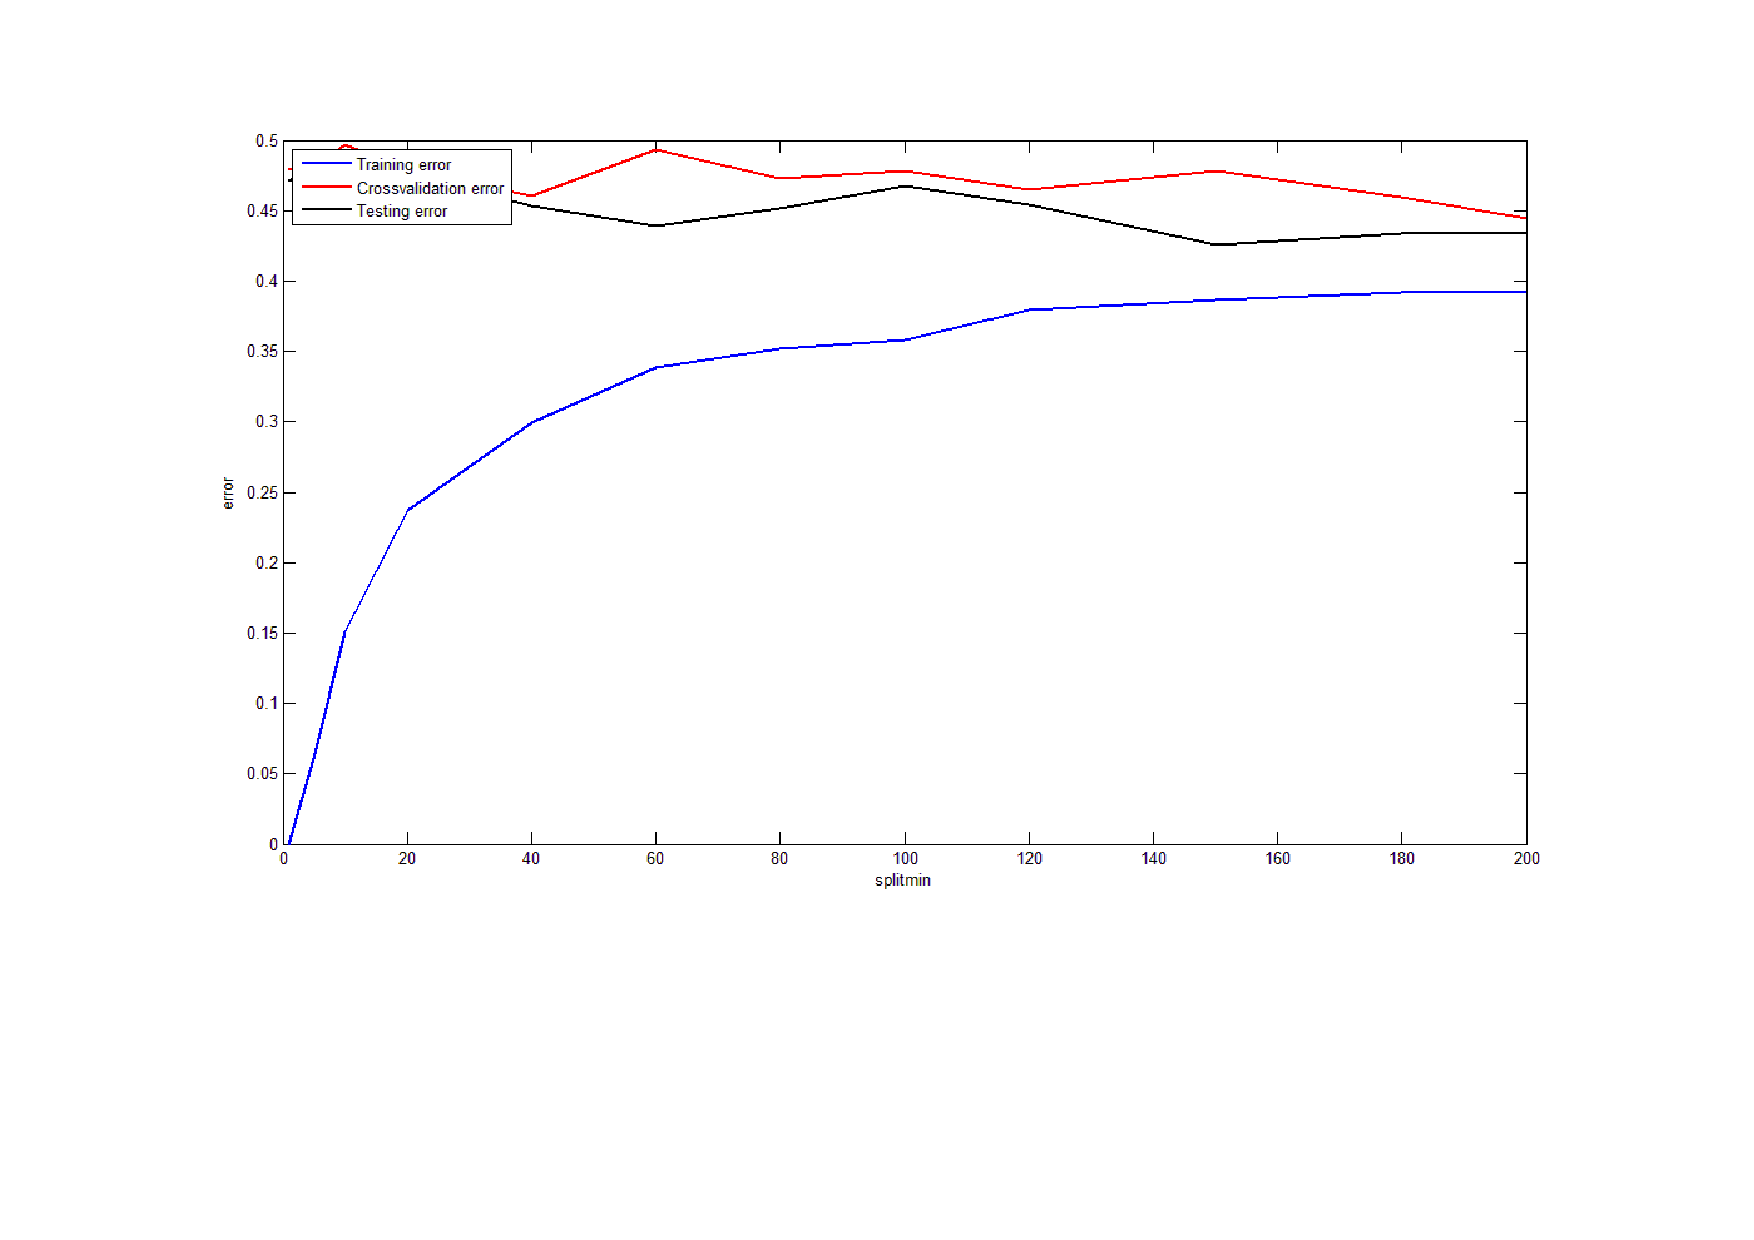
\includegraphics[width=4in]{error.pdf}
\caption{Chyba v z\'{a}vislosti na ohebnosti modelu}
\end{center}\label{f-ac}
\end{figure}
 vid\'{i}me, \v{z}e nejlep\v{s}\'{i} je vytvo\v{r}it tr\'{e}novac\'{i} mno\v{z}inu z asi 75\% dat.


\begin{figure}[!h]
\begin{center}
\includegraphics[width=4in]{linearingcurve.pdf}
\caption{U\v{c}\'{i}c\'{i} k\v{r}ivka.}
\end{center}\label{f-ac}
\end{figure}

\begin{figure}[!h]
\begin{center}
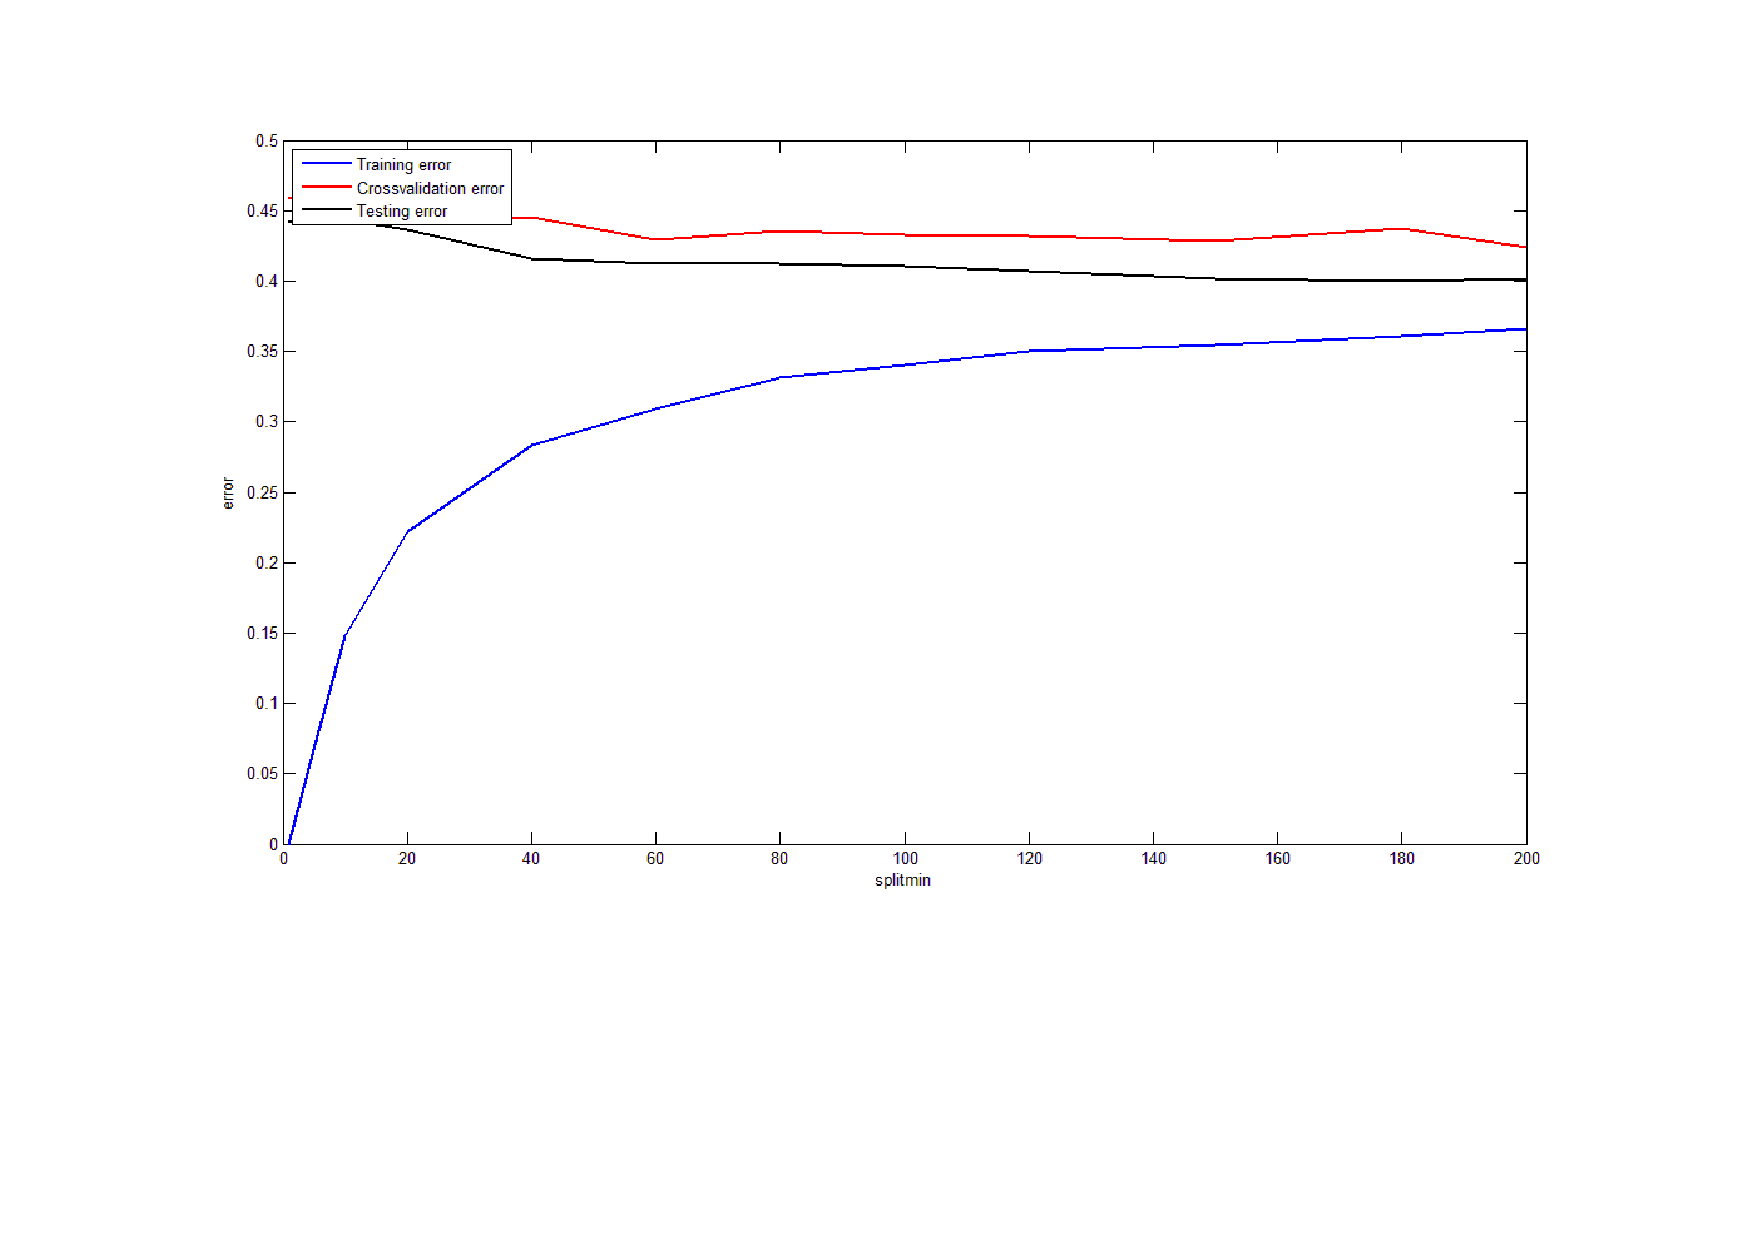
\includegraphics[width=4in]{untitled.pdf}
\caption{Druh\'{y} pokus chyby}
\end{center}\label{f-ac}
\end{figure}


\section{Conclusion}
Zjistil, \v{z}e je nejv\'{y}hodn\v{e}j\v{s}\'{i} vybrat do tr\'{e}novac\'{i} mno\v{z}iny 75 \% dat. Parametr splitmin je nejv\'{y}hodn\v{e}j\v{s}\'{i} pro hodnotu 60.
\begin{literatura}{1}

\bibitem{IEEEhowto:kopka}
Materi\'{a}ly z p\v{r}edn\'{a}\v{s}ek.

\end{literatura}

\end{document}


